\subsubsection{Chequeo de diferencias con Audacity}
\label{subsec:chequeo-diferencias}
Para poder verificar si hay diferencias entre dos archivos de audio en Audacity, es necesario proceder del siguiente modo. Con el programa abierto, se arrastran los dos archivos hacia la ventana del mismo para que sean importados automáticamente (si es la primera vez, se va a preguntar si se quiere trabajar sobre los mismos archivos, o sobre una copia temporal de los mismos; por seguridad, se recomienda elegir esta última opción, y que el programa la recuerde).\vspace{\baselineskip}

Como ambos archivos son ``de salida'' (para nuestro programa), serán los dos stereo. Es necesario separar los canales de cada uno de los archivos, para compararlos entre sí. Hacer click sobre la flecha al lado del nombre del archivo, y clickear en ``Split Stereo to Mono'' (o presionar la tecla \textbf{n}); ver figura \ref{fig:audacity-split-stereo}.


\begin{figure}[H]
    \centering
    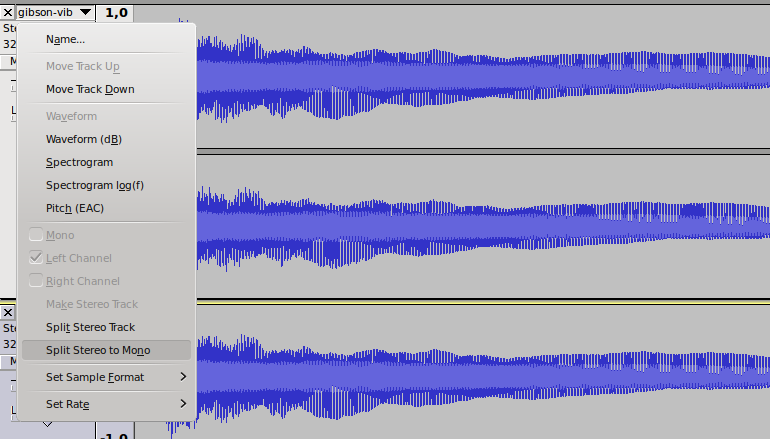
\includegraphics[scale=0.70]{imagenes/audacity-split-stereo.png}
    \caption{Convertir Stereo a canales Mono}
    \label{fig:audacity-split-stereo}
\end{figure}


Separados ya los canales de ambos archivos, seleccionar el canal izquierdo del primer archivo (aparecerá con un color diferente al resto), e ir al menú ``Effect'' (\textbf{Alt+c}), y elegir ``Invert''; ver figura \ref{fig:audacity-invert}.\vspace{\baselineskip}

\begin{figure}[H]
    \centering
    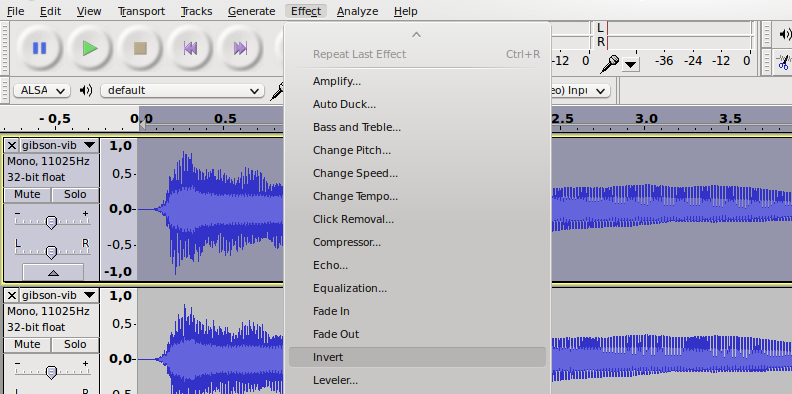
\includegraphics[scale=0.68]{imagenes/audacity-invert.png}
    \caption{Invertir canal}
    \label{fig:audacity-invert}
\end{figure}

Invertido, por ejemplo, el canal izquierdo del primer archivo, se selecciona dicho canal, junto con el izquierdo del segundo archivo (\textbf{shift+click} en los cuadrantes grises a la izquierda de cada señal). Con los dos canales correspondientes seleccionados, uno de ellos invertido, se va al menú ``Tracks'' (\textbf{Alt+t}), y se selecciona la opción ``Mix and Render'' (tecla \textbf{x}); ver figura \ref{fig:audacity-mix-and-render}.

\begin{figure}[H]
    \centering
    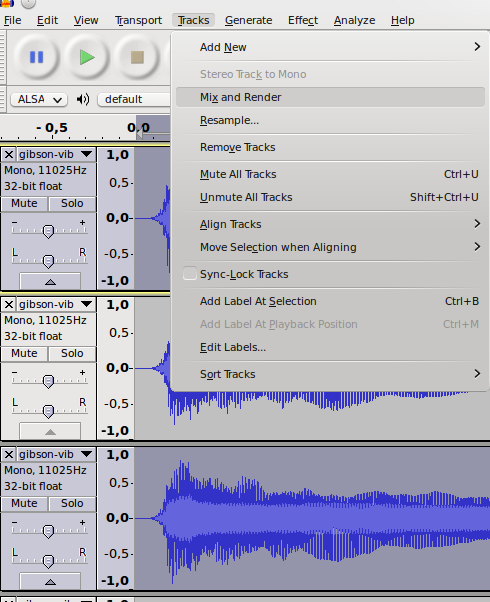
\includegraphics[scale=0.70]{imagenes/audacity-mix-and-render.png}
    \caption{Mix and render}
    \label{fig:audacity-mix-and-render}
\end{figure}

Los dos canales seleccionados que fueron mezclados, originalmente tenían la misma información. Al invertir uno de ellos, y mezclarlos entre sí, se produce una cancelación de la onda. Por lo tanto, si efectivamente contenían la misma información, debería verse el nuevo canal generado completamente vacío; ver figura \ref{fig:audacity-no-wave}. Durante el desarrollo del \textbf{TP}, esto a veces se consiguió y otras no, y las razones de ello se verán en las secciones correspondientes.

\begin{figure}[H]
    \centering
    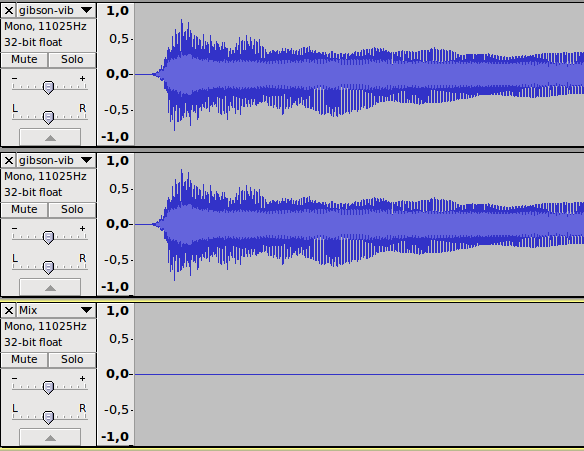
\includegraphics[scale=0.70]{imagenes/audacity-no-wave.png}
    \caption{Cancelación de la onda}
    \label{fig:audacity-no-wave}
\end{figure}

El canal izquierdo es la señal seca; repetir luego el mismo procedimiento con los dos canales derechos restantes. 
